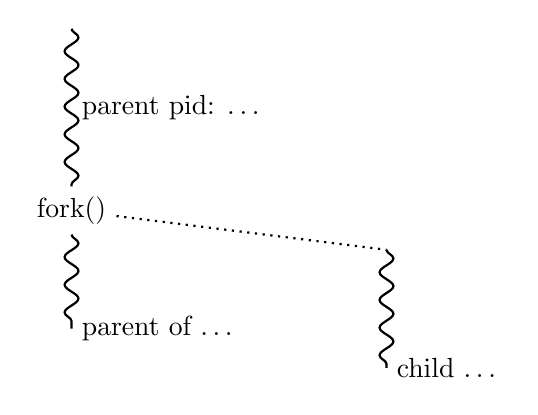
\begin{tikzpicture}
\tikzset{
    thread/.style={decoration={snake},decorate,thick},
}
\coordinate (thread start) at (0, 0);
\draw[thread] (thread start) -- ++(0, -2) node[below] (fork) {fork()} node[midway,right] {parent pid: \ldots};
\draw[thread] (fork) -- ++ (0, -1.5) node[right]{parent of \ldots};
\draw[thick,dotted] (fork) -- ++(4, -.5) coordinate (new thread start);
\draw[thread] (new thread start) -- ++(0, -1.5) node[right] {child \ldots};
\end{tikzpicture}
